This chapter covers the modelling of the building blocks of the robot.

\section{Problem statement}
Our robot will be made from a number of elements that all need to be represented in the simulation :\begin{itemize}
\item servos
\item cameras
\item hands, feet
\item electronics
\end{itemize}
We will first model the inactive elements such as the feet or the electronics before modelling the active elements, servos and cameras.

\subsection{Convex elements}
A convex element is an element whose interior angles are all less or equal to $180\degree$. Our humanoid robot will have some number of them since a lot of elements can be approximated as cubes, which are convex.

The modelling consists in creating a mesh with the right dimensions, setting the mass and setting the inertia (V-Rep does not feature matrix inertias, only principal axes inertias). Friction of the material can also be set and will influence how much an object will slide.

\subsection{Concave elements}
A shape is concave if it is not convex. It is not recommended to use concave shapes in a simulation as they make collision detection more expensive and the simulation is generally more unstable. 

Therefore, it is best to approximate such a shape by a convex mesh whenever possible. If not, then we separate it into several convex shapes that we group together with constraints.

\section{Modelling the inactive elements}

\begin{table}[htp]
\center
\begin{tabularx}{\textwidth}{@{} l X X l @{}}
\toprule
\textbf{Module} & \textbf{Weight [$g$]} &  \textbf{Density [$kg/m^3$]}& \textbf{Dimensions [$mm \times mm \times mm$]}\\ 
\midrule
Odroid C-2 & 40 & 840 & 85.0 x 56.0 x 10.0\\
Li-Po battery & 188 & 2304 & 103.0 x 33.0 x 24.0\\
Mx-28R & 72 & 1150 & 35.6 x 50.6 x 35.5\\
Hand & & & 70.0 x 31.0 x 31.0\\
Feet & & & \\
\bottomrule
\end{tabularx}
\caption[Weights and dimensions of the pieces of the robot]{Weights and dimensions of the pieces of the robot. The density is useful for the automatic computation of the weight and inertia of the pieces in V-REP.}
\label{table:weights}
\end{table}

\subsection{Electronics}
By electronics we mean the motherboard and the power electronics. The motherboard is an Odroid C-2, shown in \cref{fig:electronics}. It is intended to be the sole CPU onboard the robot. The role of the power electronics will be to convey the energy stored in the batteries to the servo motors. 

\begin{figure}[htp]
\center
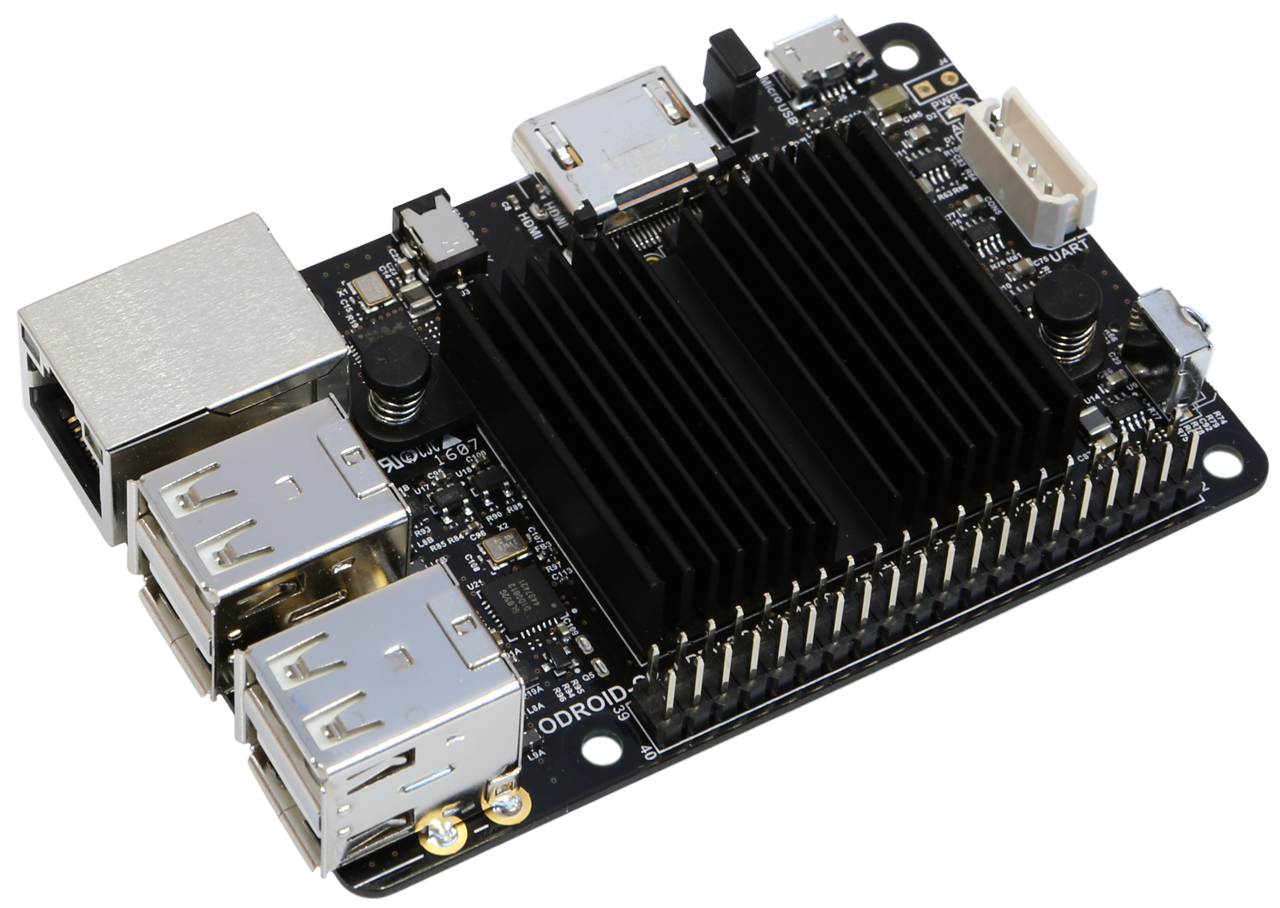
\includegraphics[width=0.3\textwidth]{figures/odroid-c2}
\caption[Odroid C-2 motherboard]{Odroid C-2 motherboard. Equipped with an ARM 2GHz quadcore CPU and 2GB of DDR3 RAM.}
\label{fig:electronics}
\end{figure}

As of now, only the size of the motherboard is known to us, as the power electronics are not yet ready. Nevertheless, a rough guess can be made : we will assume that the electronics will take twice the volume of the Odroid C-2. That volume is represented as a cube, of dimensions and size compiled in \cref{table:weights}.

\subsection{Hands}
We call \emph{hands} the elements that will mimic human hands. As the Robocup competition does not require to manipulate objects, the hands may well be simple tubes or cubes. However, in an effort to make the robot more versatile, grippers of some kind may be used instead.

We chose to model the hands as cylinders, of dimensions and size as presented in \cref{table:weights}.

\subsection{Feet}
At the moment of writing this report, the drawings of the feet are not completed. Nevertheless we can assume that approximating them as cube will not be too far from reality. The exact dimensions and weight are shown in \cref{table:weights}.

The choice of the material to use for the feet is rather important. The friction will have some influence on the behaviour of the robot. According to the material chosen, we can modify the friction parameter of the feet.

\subsection{Central plate}
The central plate will be the main body of the robot. It will support the electronics, the batteries and the arms and legs will be attached to it.

\subsection{Frames}
In an effort to make the simulation as fast and stable as possible, frames are not physically active in the simulation. They are present, but only for visualisation purpose and do not influence the outcome of the simulation.

\subsection{Springs}
It is planned to have springs on the legs of the robot, to try and make walking more energy efficient. 

V-Rep provides an object that can represent a spring, the \emph{prismatic joint}.

\section{Modelling the active elements}
\subsection{Cameras}
The robot will be equipped with two small cameras, of the type illustrated in \cref{fig:camera}, used to locate the robot on the field\footnote{This is the subject of another master thesis this year}. 

\begin{figure}[htp]
\center
    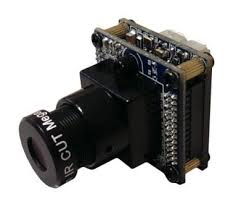
\includegraphics[width = 0.3\textwidth]{figures/li_cam}
    \caption{LI-USB30-M021C camera.}
    \label{fig:camera}
\end{figure}

We model the hull of the camera as cube. The dimensions and weight are in \cref{table:weights}. We model the active part of the camera as a \emph{vision sensor}, a V-Rep object that simulates cameras. It can be customized to have the desired resolution, field-of-view, ...

That image sensor can be reached through the remote API of V-Rep in a number of ways : \begin{itemize}
\item Streaming : the data from the vision sensor can be sent continuously to the control code but this slows down the simulation significantly. V-Rep supports streaming, reducing the communication overhead.
\item Oneshot : we can request one image from the simulator. This is less expensive and will probably be preferred.
\end{itemize} 

All the characteristics of the model of a camera are compiled in \cref{table:cam_specs}.

\begin{table}[htp]
\center
\begin{tabularx}{\textwidth}{@{}X X X @{}}
\toprule
 & \textbf{Data} & \textbf{Unit}\\ 
\midrule
Weight & 22 & $g$\\
Dimensions & 26.0 x 26.0 x 14.7 & $mm^3$\\
Inertia & & $gmm^3$\\
Resolution &  & $px^2$\\
Field of view & & $\degree$\\
\bottomrule
\end{tabularx}
\caption{Characteristics of the model of the LI-USB30-M021C camera}
\label{table:cam_specs}
\end{table}

\subsection{Servos}
\begin{figure}[htp]
\center
\begin{subfigure}[b]{0.3\textwidth}
    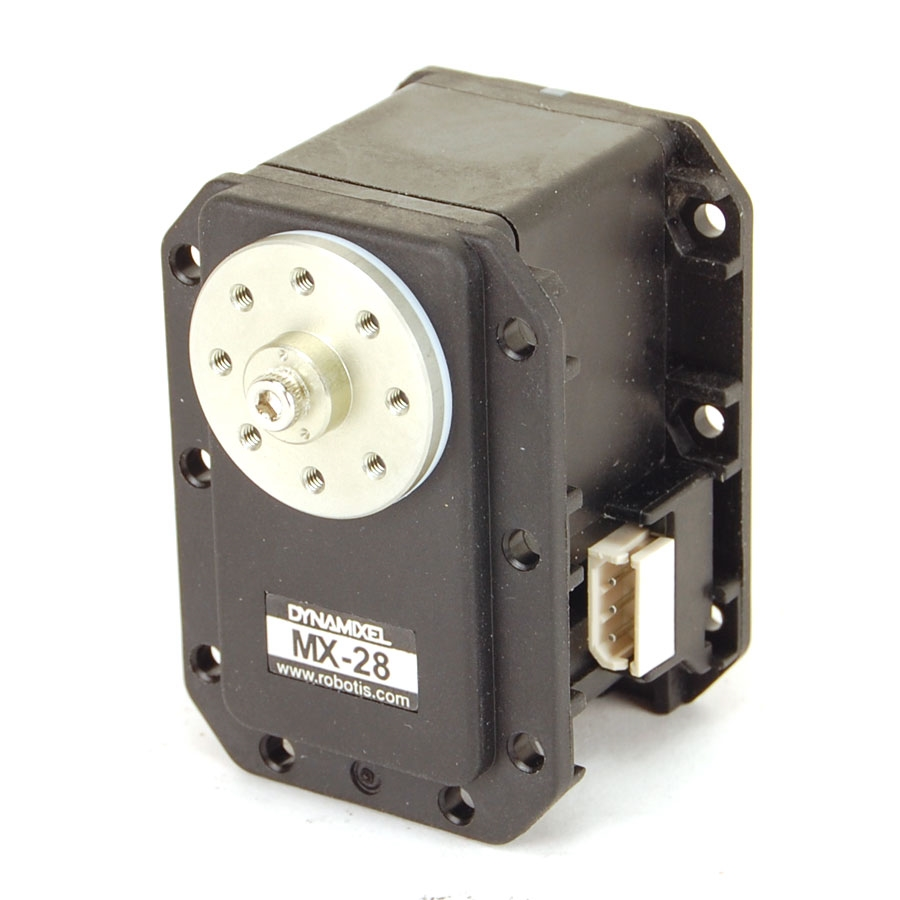
\includegraphics[width = \textwidth]{figures/mx28}
    \caption{MX-28R servo.}
    \label{fig:mx28}
\end{subfigure}
\hfill
\begin{subfigure}[b]{0.3\textwidth}
    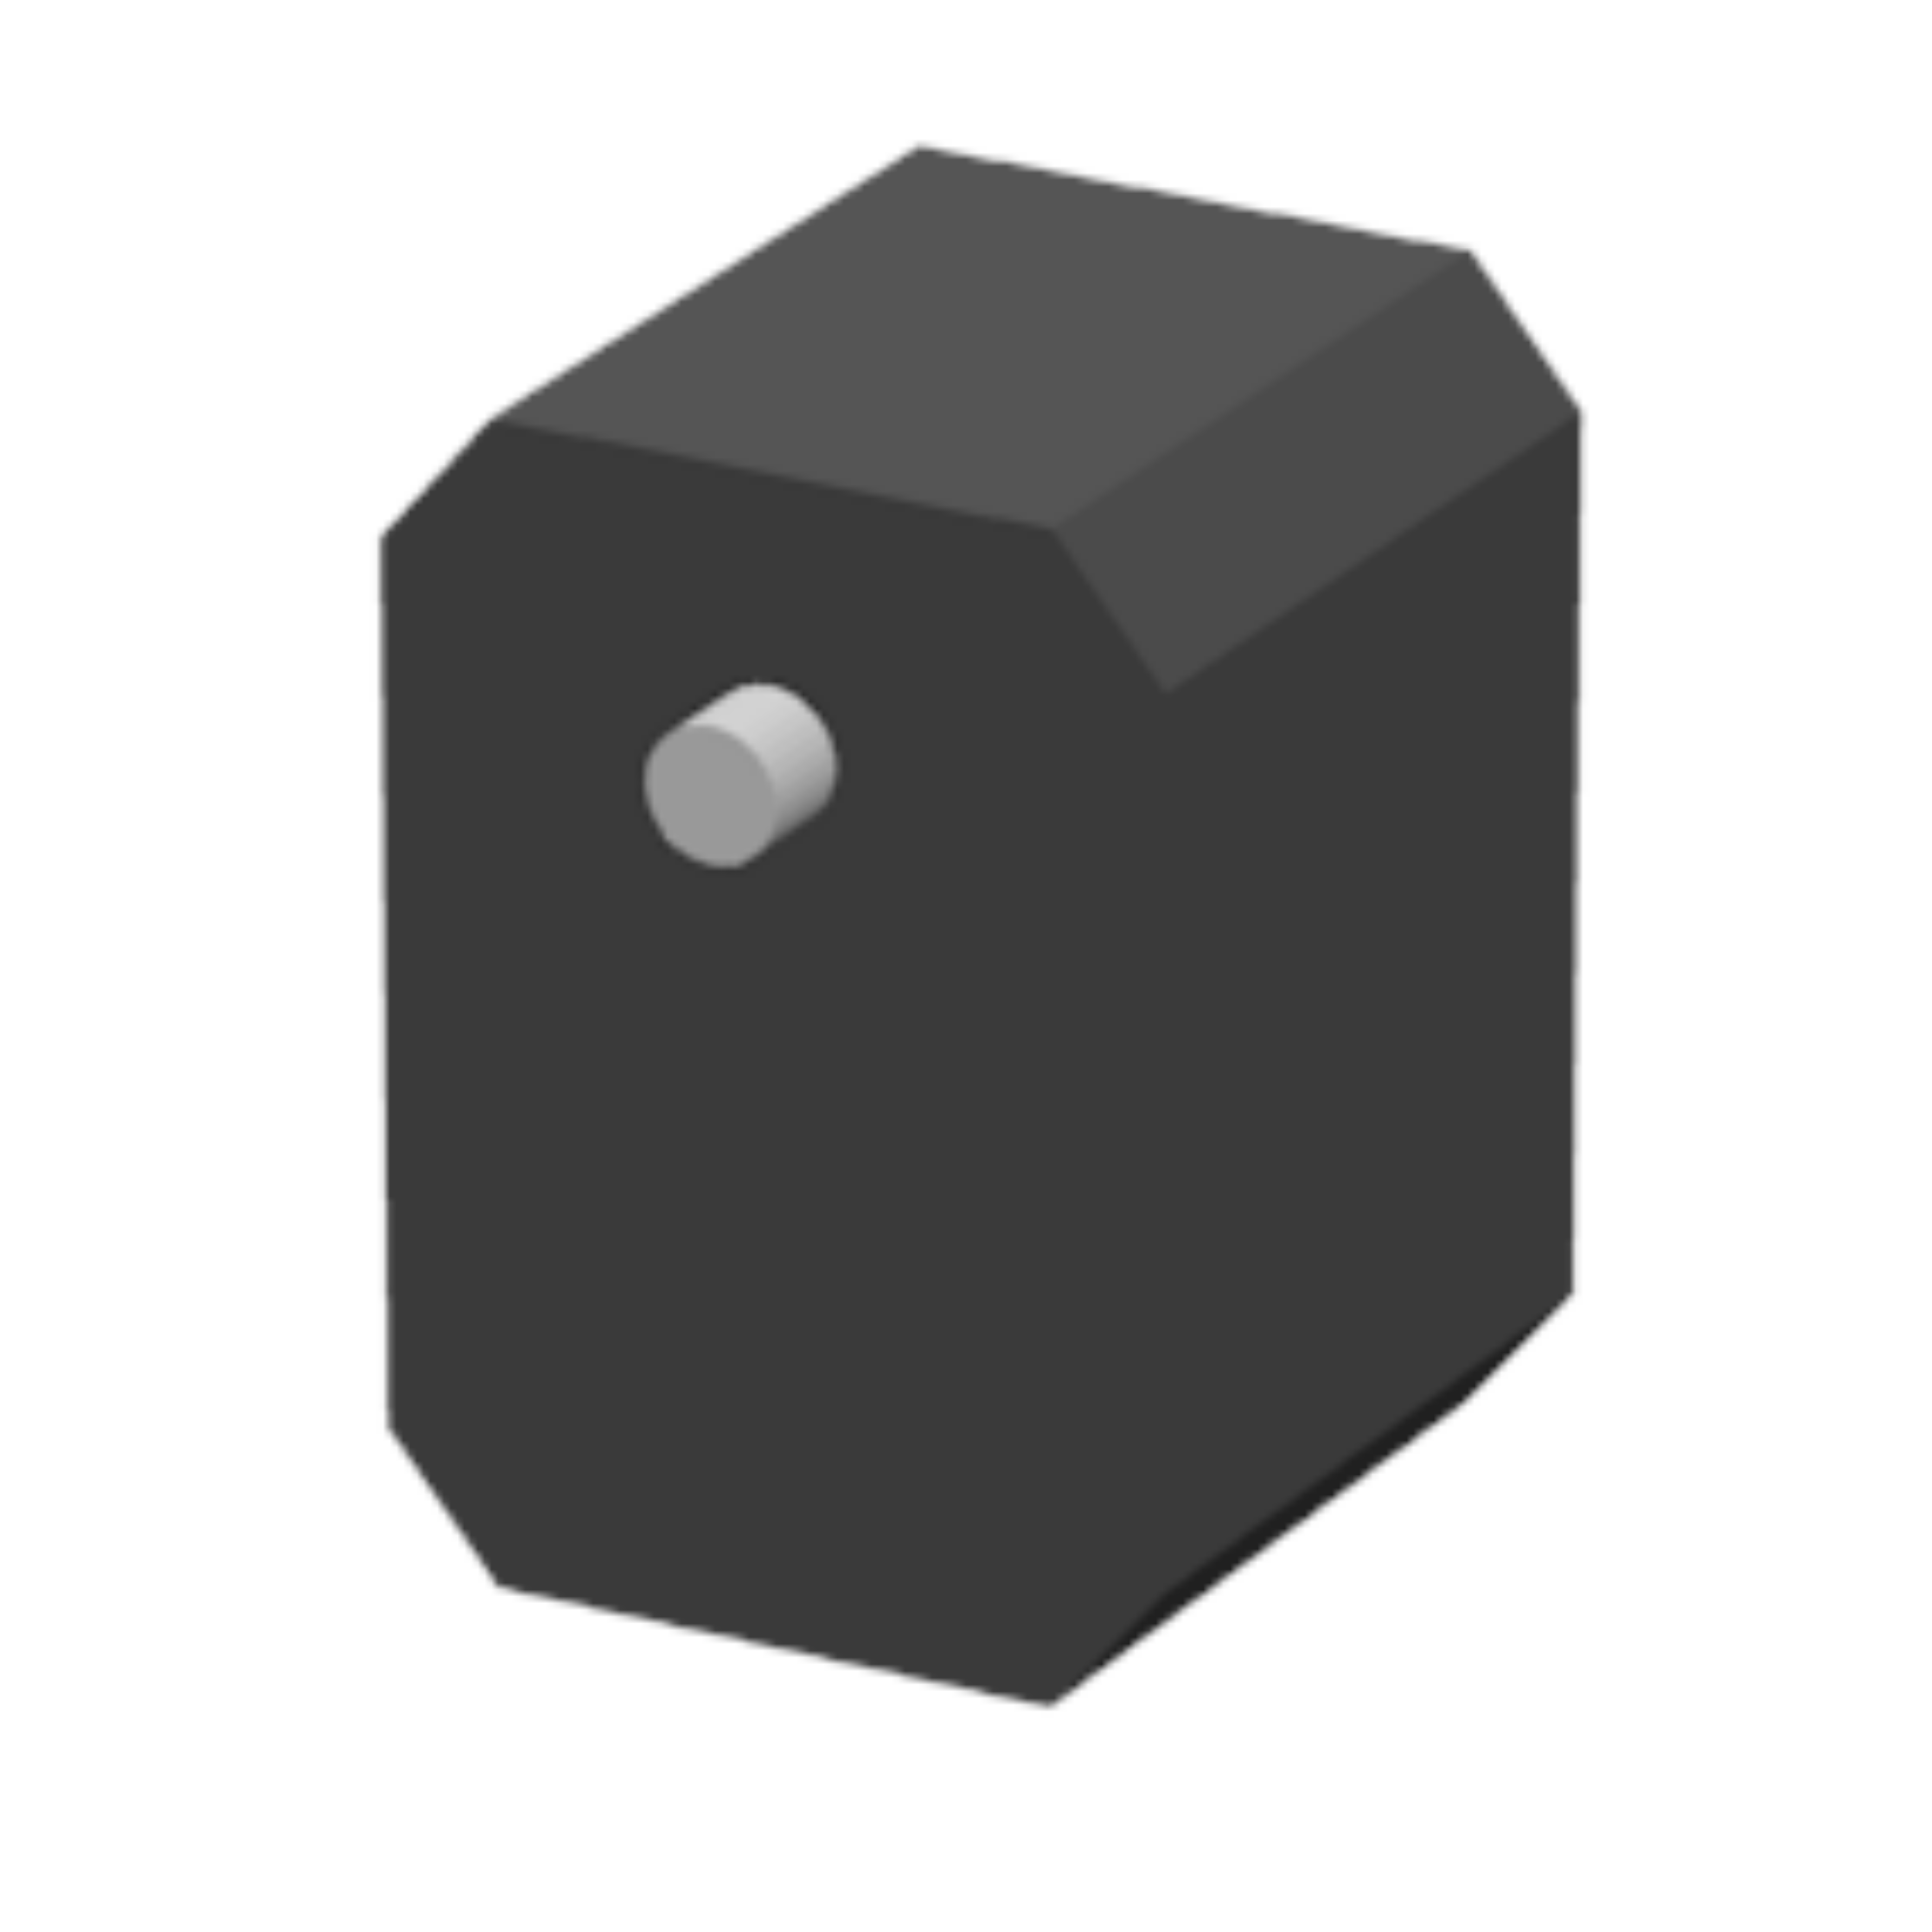
\includegraphics[width = \textwidth]{figures/mx28_model}
    \caption{Model of the MX-28R.}
    \label{fig:mx28_model}
\end{subfigure}
\caption[Side by side of a MX-28R servo and its 3D model]{Side by side of a MX-28R servo and its 3D model. The shape has been simplified but retains outer appearance of the servo. The axis is used as a position marker and will be removed once the joints are in place.}
\label{fig:servo}
\end{figure}

The robot will mainly be made from MX-28R servos (\cref{fig:mx28}) manufactured by Dynamixel. Their size and power make them an good choice for a humanoid robot. The goal of this section is thus to reproduce as accurately as possible the behaviour of this servo in our simulation. 

The MX-28R outer shape is convex so we create a convex mesh to model its appearance. As the manual \cite{mx_28_manual} does not provide the actual continuous torque, we compute from the maximal torque of the DC motor and the reduction ratio of the gears. 
\begin{align*}
Torque &= TorqueMotor \times ReductionRatio\\
&= 3.67e^{-3} \times 193\\
&= 0.7083Nm
\end{align*}

\begin{table}[htp]

The servo uses a PID controller to reach and hold a desired position. The model inside V-Rep also uses a PID and the code is in \cref{lst:servo}.

\begin{tabularx}{\textwidth}{@{} l l X @{}}
\toprule
& \textbf{Data} & \textbf{Unit}\\ 
\midrule
Weight & $77$ & $g$\\
Dimension & $35.6 \times 50.6 \times 35.5$ & $mm^3$\\
Inertia around main axes & $\begin{array}{c c c}
33,765 & 12,900 & 28,821
\end{array}$ & $g \times mm^4$ \\
Stall torque & $2.5$ & $Nm$\\
Nominal torque & $0.7$ & $Nm$\\
\bottomrule
\end{tabularx}
\caption{Characteristics of a MX-28R type servo. Data taken from \cite{mx_28_manual}}
\label{table:specs}
\end{table} 

The original MX-28R servo does not have any accelerometry, but a master thesis in progress is going to change that. We can emulate it in the simulator by differentiating the position, obtained through \emph{simxGetObjectPosition}. 